\chapter{Efficient solution of the linear systems}
\chaptermark{Solution of linear systems}
\label{sec:solution-strategies}

\newcommand{\Nn}{N} % nnodes
\newcommand{\Nb}{N_b} % boundary nodes
\newcommand{\Nj}{N_j} % jacobian rows

When we combine implicit time integration schemes, a FEM spatial discretisation and the Newton-Raphson method for linearisation (as discussed in \cref{sec:time-discretisation,sec:galerk-meth-llg}) we are left with a sequence of sparse linear systems which must be solved to obtain the approximate solution.
With the addition of FEM/BEM for calculation of magnetostatic fields (as discussed in \cref{sec:hybr-finit-elem}) the linear systems to be solved become larger and more complex.
In this \thisref{sec:solution-strategies} we discuss solution strategies for these systems.

In \cref{sec:llg-only-system} we first discuss the solution of the systems required in the calculation of the magnetostatic field assuming the magnetisation is known.
We then discuss methods of solving the linear systems for the LLG equation assuming the magnetostatic field is known.

In \cref{sec:solut-coupl-syst} we introduce methods for the solution of the combined system: the LLG equation with magnetostatics, this process is complicated by the inclusion of the dense BEM matrix.
In particular, in \cref{sec:fully-implicit-bem}, we introduce a novel approach which can efficiently solve the coupled system while retaining all properties of the original time integration scheme.

Finally in \cref{sec:numer-exper-fem-bem-systems} we present some numerical experiments comparing the approaches.


\section{Solution of decoupled systems}
\label{sec:llg-only-system}

??ds should the libraries and parameters used go in implementation section? If you move it make sure you add the other section when referencing from numerical experiments

In \thisref{sec:llg-only-system} we consider the separate solution of the magnetostatic and LLG problems.
Such methods are important building blocks for the solution of the coupled system.

First the two linear systems solved in the magnetostatic field calculations: these both are Poisson systems (see \cref{sec:poisson-jacobian}), which are extremely well studied.
One efficent and robust method for solving Poisson systems on unstructured grids is to use the method of conjugate gradients (CG) with algebraic multigrid (AMG) as a preconditioner \cite[Chap. 2]{HowardElmanDavidSilvester2006}.
We implement such a solver using \oomph's implementation of CG with a relative convergence tolerance of $10^{-8}$.
As the preconditioner we use one V(1,1) cycle of \hypre's BoomerAMG preconditioner \cite{hypre} with Gauss-Seidel smoothing, CLJP coarsening and a connection strength threshold of $0.7$.

Note that the Poisson blocks $\Am$ do not depend on $\phim$, $\phione$ or $\mv$ (\ie the Poisson problems are linear).
This means that when solving these matrices the Newton-Raphson iteration is not required (or if used it will converge in a single iteration assuming that the linear solve is sufficiently accurate).
Also the $\Am$ matrices only depend on the geometry and so can be computed once and stored for reuse throughout the duration of the simulation.


Now we focus on the sequence of linear systems resulting from solving the LLG equation with the Newton-Raphson method.
There do not appear to be any efficient, robust, and scalable solvers in the literature for this system (previously used approaches are discussed in \cref{sec:linear-solv-micr}).
We try two solvers in our implementation, unfortunately neither are expected to be scalable to large problem sizes with large time steps.

The first method used is a direct solve by LU decomposition (using the \superlu package \cite{superlu}).
As discussed in \cref{sec:direct-methods} this method is extremely robust but is very slow for large matrices, particularly for problems in three spatial dimensions.

The second method is to use a Krylov solver preconditioned by an incomplete LU decomposition (ILU), inspired by \cite{Suess2002}.
We \oomph's GMRES implementation with left preconditioning, no restarts and a relative convergence tolerance of $10^{-8}$.
For the ILU preconditioner we use \hypre's Euclid with one level of fill in and no drop tolerance.
Incomplete LU decomposition with no fill in was also tested but found to be ineffective, especially for larger time steps.
This method is expected to be efficient for medium sized problems and/or small time steps, especially in 2D or thin film problems where there is less coupling FEM nodes.
However it is not expected to scale to large meshes or to be robust with respect to varying parameters.
??ds mention why small steps?: diagonally dominant, why small nnode?

Unfortunately we have not had time to research more effective solvers for the LLG system.

\section{Solution of coupled LLG-magnetostatics systems}
\label{sec:solut-coupl-syst}

We now need to consider the solution of the combined LLG and FEM/BEM magnetostatics systems.
However, unlike typical FEM computations, these linear systems are not entirely sparse.
The BEM matrix, $\bm$, (derived in \cref{sec:discretisation}) appears as a dense block in the Jacobian.
In this \thisref{sec:semi-implicit-bem} we describe two approaches to efficiently solve the non-linear system despite this issue.

The first approach involves replacing our implicit time integration scheme with an ad-hoc semi-implicit version which handles the magnetostatic calculation explicitly.
This means that only decoupled solves for $\phione$, $\phi$ and $\mv$ are required at each time step, and the dense block only appears as a matrix-vector multiply.
However it also means that we are no longer using the time integration methods discussed in \cref{sec:some-implicit-time-integrators}, instead we are using some new and unknown scheme.

The second approach is to construct a linear solver which can efficiently handle the dense block.
We present a novel solver which consists of a Krylov solver combined with a block preconditioner, iterative subsidiary solves and a hierarchical representation of the BEM block.
This approach has the benefit that all of the properties of the original time integration schemes carry over to the coupled problem.
In particular, when using this approach but not when using a semi-implicit approach, the IMR retains the energy property described in \cref{sec:proof-energy-prop}, which is the most unique of its geometrical integration properties.\footnote{A number of explicit integration schemes can obtain length conservation: Cayley transform methods \cite{Lewis2003}, semi-analytical methods \cite{Wiele2010} and various types of semi-implicit midpoint rule methods \cite{Spargo2003} \cite{Mentink2010} (including the one described in \thisref{sec:solution-strategies}).}
Additionally it may be useful for stochastic problems (\ie when thermal fields are involved, see \cref{sec:temperature-effects}), in this case only a few time integration schemes are known to converge to the correct solution \cite{DAquino2006}.
The implicit midpoint rule is one of these schemes, but the semi-implicit modification is likely to remove this property

Before describing these approaches in more detail we briefly discuss how the coupling can be implemented and the structure of the Jacobian for the coupled LLG-magnetostatics problem.

\subsection{Residuals and Jacobian for the coupled system}
\label{sec:bem-jacobian-structure}

As mentioned in \cref{sec:discretisation} contribution of the pair of potentials used in the FEM/BEM method is similar to that of the simplified magnetostatic potential discussed in \cref{sec:galerk-meth-llg}.
There are two differences, the first is that there is no coupling from the auxiliary potential $\phione$ to the LLG equation, and hence no corresponding $\Pm$ block.

The second difference is that there is an additional coupling between the boundary values of $\phione$ and the boundary values of $\phim$.
This coupling between the BEM part (a collocation method) and the FEM part (a Galerkin method) is implemented using the following vector of residuals (one residual for each boundary node)
\newcommand{\rphimb}{\rphi_b}
\begin{equation}
  \rphimb(\phimdis_b, \phionedis_b) = \bm \phionedis_b - \phimdis_b,
  \label{eq:89}
\end{equation}
where $\mydiscrete{x}_b$ denotes the vector of values of $x$ at the boundary nodes.
This residual is included as normal in the non-linear solve and simply enforces the condition $\phimdis_b = \bm \phionedis_b$ from \cref{eq:10}.
Note that we cannot enforce the condition in the standard way (by setting the boundary values of the solution basis functions) because the condition to be enforced is determined as part of the solve.

A natural consequence of \cref{eq:89} is that the BEM matrix is a block of the Jacobian:
\begin{equation}
  \pd{\rphimb}{\phionedis_b} = \bm,
\end{equation}
where we have again used the notation that $\pd{\av}{\bv}$ is the Jacobian of the derivatives of $\av$ with respect to $\bv$, as in \cref{eq:jac-def}.
Also note that the diagonal Jacobian block for the boundary values of $\phim$ is
\begin{equation}
  \pd{\rphimb}{\phimdis_b} = -\Idm.
\end{equation}

Combining these points with the Jacobian matrix derived in \cref{sec:llg-magn-coupl} the complete Jacobian is
\begin{equation}
  \Jm =
  \begin{pmatrix}
    \Fm       & \Pm     &  \\
    \Qm'      & \Am' &  \bm'  \\
    \Qm       &         &   \Am
  \end{pmatrix},
  \label{eq:16}
\end{equation}
where the order of blocks is $\mv$, $\phim$, $\phione$ and primed blocks are those where the boundary and bulk values must be split up because of the BEM coupling:
\begin{equation}
  \Am' =
  \begin{pmatrix}
    \Am     & \pd{\phimh}{\phimdis_b} \\
    0      & -\Idm
  \end{pmatrix},
  \qquad
  \Qm' =
  \begin{pmatrix}
    \Qm \\
    0
  \end{pmatrix},
  \qquad
  \bm' =
  \begin{pmatrix}
    0  & 0 \\
    0  & \bm
  \end{pmatrix},
\end{equation}
where the bulk values are the first blocks and the boundary values the second.

??ds think I need to mention sizes of blocks, how should I do it?
Need to make sure I introduce $\Nn$ = n nodes, $\Nj$ = n rows and $\Nb$ = n boundary nodes.
Also I don't really like the prime notation here...

It is worth noting that a slightly different Jacobian struture could be obtained by modifying the derivation in \cref{sec:appl-magn-calc}.
Instead of using $\phim = \phione + \phitwo$ to eliminate $\phitwo$, we could use $\hms = - \grad ( \phione + \phitwo)$ and eliminate $\phim$.
This would result in both of the potentials having a $\Pm$ block, but only one of them having a $\Qm$ block.
It would also reduce the diagonal dominance of $\bm$.
We have not experimented with this alternative formulation.

The linear system to be solved at each Newton step is (see \cref{sec:newt-raph})
\begin{equation}
  \jac \corr = -\resi,
  \label{eq:87}
\end{equation}
where $\resi$ is the vector of the current discrete Newton residuals for $\mv$, $\phim$ and $\phione$ and we need to find the Newton update $\corr$.


\subsection{The semi-implicit approach}
\label{sec:semi-implicit-bem}

One approach to the solution of the linear system \cref{eq:87} is to break it into multiple decoupled systems.
The idea is to use implicit calculations for the LLG parts as normal, but to treat the magnetostatic calculations explicitly.
Since the magnetostatic fields are typically much weaker than the exchange field we hope that the stability of the scheme will not be greatly reduced.

An outline of the algorithm for the step from time $t_n$ to $t_{n+1}$ is as follows
\begin{enumerate}
\item Extrapolate the magnetostatic potential (using $\phim_n$, $\phim_{n-1}$) to time $t_{n+1}$, and call the result $\hat{\phim}_{n+1}$.
\item Use the explicit approximation $\hat{\phim}_{n+1}$ to calculate $\mv_{n+1}$ using an implicit time integration scheme.
\item Calculate $\phione_{n+1}$ using $\mv_{n+1}$ (Poisson solve).
\item Use boundary values of $\phione_{n+1}$ to get $\phim_{n+1}$ on the boundary (BEM matrix-vector multiply).
\item Calculate $\phim_{n+1}$ everywhere using the dirichlet boundary conditions given by 4. and $\mv_{n+1}$ (Poisson solve).
\end{enumerate}
Note that we use an extrapolation of the magnetostatic potential to $t_{n+1}$ rather than using a step of an explicit time integration scheme because there is no time derivative in the equations for $\phim$.
Alternatively we could take an explicit step of the LLG and use this to calculate $\hat{\phim}_{n+1}$. ??ds would that be any better? more stable maybe?

For step 1 we require a second order accurate extrapolation in order to ensure that the local truncation error of the overall time integration scheme remains second order.
A simple second order extrapolation formula (based on Lagrange interpolation \cite[312]{Kincaid2002}) is
\begin{equation}
  \label{eq:65}
  f(t_{n+1}) = \frac{t_{n+1} - t_n}{t_{n-1} - t_n}f(t_{n-1}) + \frac{t_{n+1} - t_{n-1}}{t_n - t_{n-1}}f(t_n),
\end{equation}
replacing differences in time with the appropriate time steps this gives
\begin{equation}
  \label{eq:66}
  \hat{\phim}_{n+1} = \frac{-\dtx{n+1}}{\dtn} \phim_{n-1} + \frac{\dtx{n+1} + \dtn}{\dtn} \phim_n.
\end{equation}
Note that if we are using the implicit midpoint rule we need to extrapolate $\phim$ to the midpoint rather than $t_{n+1}$, hence we use $\dtx{n+1} = \dtx{n+1} /2$ in the above equation.

??ds write out LTE for this scheme somehow?

Unfortunately this method requires two initial values for the magnetostatic potential values to start.
The additional value can be generated by directly calculating the potential if the magnetisation values at two initial times are known.
Otherwise the first can be calculated from the initial condition and the potential at a second time can be calculated by taking a small time step using a first order extrapolation formula.

The linear systems resulting from the application of this algorithm are exactly those discussed in \cref{sec:llg-only-system}.


??ds mention semi-implicit + fixed point iteration approach? No one's ever used it in micromagnetics as far as I know.


\subsection{The fully implicit approach}
\label{sec:fully-implicit-bem}

The alternative to the semi-implicit approach described above is to find an efficient way to solve the full system \cref{eq:16,eq:87}, this is known as a ``monolithic'' approach.
The major difficulty is that the system contains a dense block, meaning firstly that an LU decomposition of J will be significantly more dense than for a typical FEM Jacobian.
Secondly this means that any operations (\eg multiplication) on J will be significantly slower than for a sparse Jacobian, $\order{\Nj + \Nb^2}$ rather than $\order{\Nj}$.
We use a combination of techniques to remove or reduce these negative effects of the BEM block.

The first and most important technique is the use of a Krylov solver, this has two benefits with regards to the dense block.
Firstly the LU decomposition (nor any other representation of the inverse) of the matrix is never computed, meaning that the fact that the ``inverse'' is more dense has no effect.
Secondly, using a Krylov solver rather than a direct solve or a multigrid-based solver means that all that is required of $\jac$ is the computation of matrix-vector products.
This allows us to split $\jac$ into separate matrices as
\begin{equation}
  \jac = \jac_{\textrm{sparse}} + \Gm'',
\end{equation}
where $\Gm''$ contains only the dense block $\Gm$ and $\jac_{\textrm{sparse}}$ is sparse.
The matrix-vector product can be computed as
\begin{equation}
  \jac \xv = \jac_{\textrm{sparse}}\xv + \Gm''\xv,
\end{equation}
\ie the dense and sparse parts can be stored and used completely independently.

This leads us to the second component of our method: the use of a hierarchical matrix format for the BEM block \cite{Borm2003,Forster2003,Knittel2011}.
This format reduces the computational cost for a matrix-vector product for the dense block to $\order{\Nb \log \Nb}$.
Since the number of boundary nodes $\Nb$ is typically less than the total number of nodes in the problem this can allow the cost of matrix-vector products of $\jac$ to be optimal (\ie $\order{\Nj}$) depending on the geometry.
It also reduces the memory requirements for the block to $\order{\Nb \log \Nb}$.
The use of such formats has recently become fairly common in the application of the hybrid FEM/BEM method to micromagnetics problems.

The third and final component in our efficient solver is a cheap and effective preconditioner for the linear system.
Some approaches to constructing such a preconditioner will be discussed in the following section.


\subsubsection{Preconditioning strategies}
\label{sec:bem-solver-strategies}

\newcommand{\preca}{\mathcal{P}}
\newcommand{\precb}{\mathcal{Q}}
\newcommand{\precc}{\mathcal{R}}


\newcommand{\inexact}[1]{\widetilde{#1}}
\newcommand{\parinexact}[1]{\hat{#1}}
\newcommand{\pbin}{\inexact{\precb}}
\newcommand{\pcin}{\inexact{\precc}}




In this section we give a number preconditioning approaches for the monolithic system with the Jacobian as given in \cref{eq:16}.
The aim is to construct a preconditioner which give a (roughly) constant number of Krylov solver iterations independently of all problem parameters (and in particular independently of $\Nn$) but which is also quick to set up and does not consume a large quantity of memory.
We make some progress towards this goal, but more research is still needed.

The first preconditioner is very simple: we use a direct solve (using LU decomposition) of the sparse part of $\Jm$, \ie
\begin{equation}
  \preca =
  \begin{pmatrix}
    \Fm       & \Pm     &  \\
    \Qm'       & \Am'    &   \\
    \Qm       &         &   \Am
  \end{pmatrix}.
\end{equation}
This preconditioner, while much more efficient than a direct solve including the dense block, still suffers from all the usual problems associated with a direct solver (\ie expensive in both memory and computation time when $\Nn$ is large).
However, we are interested in its properties as a test of the effectiveness of dropping the $\Gm'$ block from the preconditioner.

As discussed in \cref{sec:linear-solv-micr} a number of other FEM/BEM based models use an approach similar to preconditioner $\preca$ \cite{Suess2002}, except that the preconditioner is solved by inner Krylov solver rather than a direct solve.
This makes the computational cost feasible for realistic problems, but has two issues:
The first is that technically an inner Krylov solve cannot be used as a preconditioner because it does not apply the same operation at each step of the outer solve (see \cref{sec:preconditioners}), this issue can be resolved by using an outer Krylov solver known as Flexible GMRES which accounts for this \cite{Saad1993}.
The second issue is that a full inner Krylov solve is run at \emph{every iteration} of the outer Krylov solve, which is computationally expensive.

Our second and third preconditioners are more ambitious: we drop additional blocks in order to make the preconditioner block triangular.
It can then be solved by inverting only the diagonal blocks (exactly or approximately) and using back/forward substitution.
The two preconditioners are
\begin{equation}
  \precb =
  \begin{pmatrix}
    \Fm       &           &  \\
    \Qm'       & \Am'&   \\
    \Qm       &           &   \Am
  \end{pmatrix},
  \qquad
  \precc =
  \begin{pmatrix}
    \Fm       & \Pm       &  \\
    & \Am' &   \\
    \Qm       &           &   \Am
  \end{pmatrix},
  \label{eq:ms-block-prec-drop-p}
\end{equation}
where the blocks in $\precc$ can be reordered to give a block triangular matrix but we write them in the normal order for consistency.
However, inverting $\precb$ or $\precc$ directly would still require an expensive, in terms of both memory and set up time, direct solve of the three diagonal blocks $\Fm$, $\Am'$ and $\Am$.
Ideally we want to approximate these inverses by some cheap iterative process instead.

Based on the fact that AMG is known to be an extremely effective preconditioner for Krylov solves of Poisson problems, we test the use of an AMG preconditioner for the $\Am$ blocks.
Using this approximation we define two partially-iterative preconditioners
\begin{equation}
  \parinexact{\precb} =
  \begin{pmatrix}
    \Fm       &           &  \\
    \Qm'       & \inexact{\Am'} &   \\
    \Qm       &           &   \inexact{\Am}
  \end{pmatrix},
  \qquad
  \parinexact{\precc} =
  \begin{pmatrix}
    \Fm       & \Pm       &  \\
    & \inexact{\Am'} &   \\
    \Qm       &           &  \inexact{\Am}
  \end{pmatrix},
  \label{eq:ms-block-prec-drop-p}
\end{equation}
where we use $\inexact{x}$ to denote that the block is approximated iteratively.

As a final preconditioner we try approximating the $\Fm$ block using ILU-1.
However we should expect some restrictions on the matrix size and time step size similar to the case of pure-LLG solves preconditioned with ILU as discussed in \cref{sec:llg-only-system}.
We define two fully-iterative preconditioners using this approximation in addition to the AMG approximation for the Poisson blocks discussed above:
\begin{equation}
  \inexact{\precb} =
  \begin{pmatrix}
    \inexact{\Fm} &           &  \\
    \Qm'       & \inexact{\Am'} &   \\
    \Qm       &           &   \inexact{\Am}
  \end{pmatrix},
  \qquad
  \inexact{\precc} =
  \begin{pmatrix}
   \inexact{\Fm}       & \Pm       &  \\
    & \inexact{\Am'} &   \\
    \Qm       &           &  \inexact{\Am}
  \end{pmatrix}.
  \label{eq:ms-block-prec-drop-p}
\end{equation}


\section{Numerical experiments}
\label{sec:numer-exper-fem-bem-systems}

We now test the performance and robustness of the linear solvers described in \thisref{sec:solution-strategies}.
A comparison of the performance and stability of the implicit and semi-implicit time integration schemes will be performed in \cref{cha:numer-experiments}.


\subsection{Problem definition and implementation details}

In order to perform these experiments we need a simple but representative problem.
We do not use the \mumag standard problem \#4 because the hybrid FEM/BEM method for magnetostatic calculations is particularly unsuited for such thin film problems (as discussed in \cref{sec:bound-elem-meth}).

Since the majority of practical FEM micromagnetics calculations are in three dimensions our test case should also be 3D.
Also it must have sharp corners or edges, in order to include the effect of near singular integrals in the FEM/BEM method.
Based on these considerations we choose to test the solvers on a $L\times L \times L$ cube with $L=1$ exchange length.

In order to test a solver we only need model a single time step of some problem, assuming that a non-trivial initial state is chosen.
As such the initial magnetisation is chosen to be
\begin{equation}
  \mv_0(x, y, z) = \threevec{\sin(2\pi x/50) + \sin(2\pi y/50)}{\cos(2\pi x/50) + \cos(2 \pi y/50)}{1.0 - m_y - m_z}.
\end{equation}
Note that a wavelength of $50$ was chosen to ensure that even relatively unrefined meshes are able to resolve the initial state.
The problem geometry and initial conditions are illustrated in \cref{fig:cube-initial-condition}.

\begin{figure}
  \centering
  
\includegraphics[width=0.8\textwidth]{images/placeholder}
  \caption{The test problem used for the linear solvers in the state at time $t=0$.}
  \label{fig:cube-initial-condition}
\end{figure}


We use a range of damping and anisotropy parameters: $\dampc = 0, 0.01, 1$, $\kone = 0, 0.1$. ??ds I should really have done $L=1,10,100$ (equivalent to varying exchange coeff), do it if there's time.
We use zero applied field to avoid inducing accidental symmetries.
Time steps of sizes $\dtn = 0.01, 0.1, 0.5, 1.0$ are chosen, and meshes with $\Nn= 71, 791, 5631, 42461$ nodes (note that the number of rows/columns in the Jacobian is roughly 5 times the number of nodes).
We use both the nodal quadrature discussed in \cref{sec:local-nodal-integr} and a standard Gaussian quadrature.
Since the only effect of changing the time integration methods on the linear systems is a small change to the constant in the time derivative terms we only run experiments using IMR.

The solvers are run both with and without the use of a hierarchical matrix representation for the $\Gm$ block.
We use the \hlib library with patches from \nmag allowing a co-location BEM approach.
For compatibility with this library we use a tetrahedral mesh.
We use the HCA II algorithm with parameters based on those used by Knittel \cite{Knittel2011}:
$\epsilon_{ACA} = 10^{-5}$,
minimum leaf matrix size $n_{\text{min}}= 30$,
admissibility criterion $\eta = 0.25$,
polynomial interpolation order $p=4$, and
numerical quadrature order $q=3$.
We also use adaptive recompression with $\epsilon = 10^{-3}$.

All experiments are run in serial on a desktop using an Intel Core i7-3820 processor running at 3.6GHz and with 16GB of RAM.


\subsection{Results}

??ds dont split by quadrature for p2p3 iterations
??ds log plots for direct solve times?

\Cref{fig:its-ilu-decoupled} shows the mean (over a single Newton solve) number of GMRES iterations required to solve the LLG-only system using ILU-1 preconditioning (\ie with magnetostatics handled by the semi-implicit approach).
As is expected with a generic preconditioner it is effective for low-medium numbers of nodes, but becomes less effective for large problems and as the time step size increases.
% In fact for the largest $\Nn$ with the largest time steps ($\dtn = 1.0$) the solver does not converge with 400 iterations for some parameters.
Note that the plot includes all values of the physical parameters, both quadratures and both $\Gm$ block formats, but these do not appear to have a major impact on the effectiveness of the preconditioner.
The mean preconditioner setup times this preconditioner are shown in \cref{fig:times-ilu-decoupled}.
As with the iteration counts, the setup times become significantly larger as $\Nn$ grows.

\begin{figure}
  \centering
  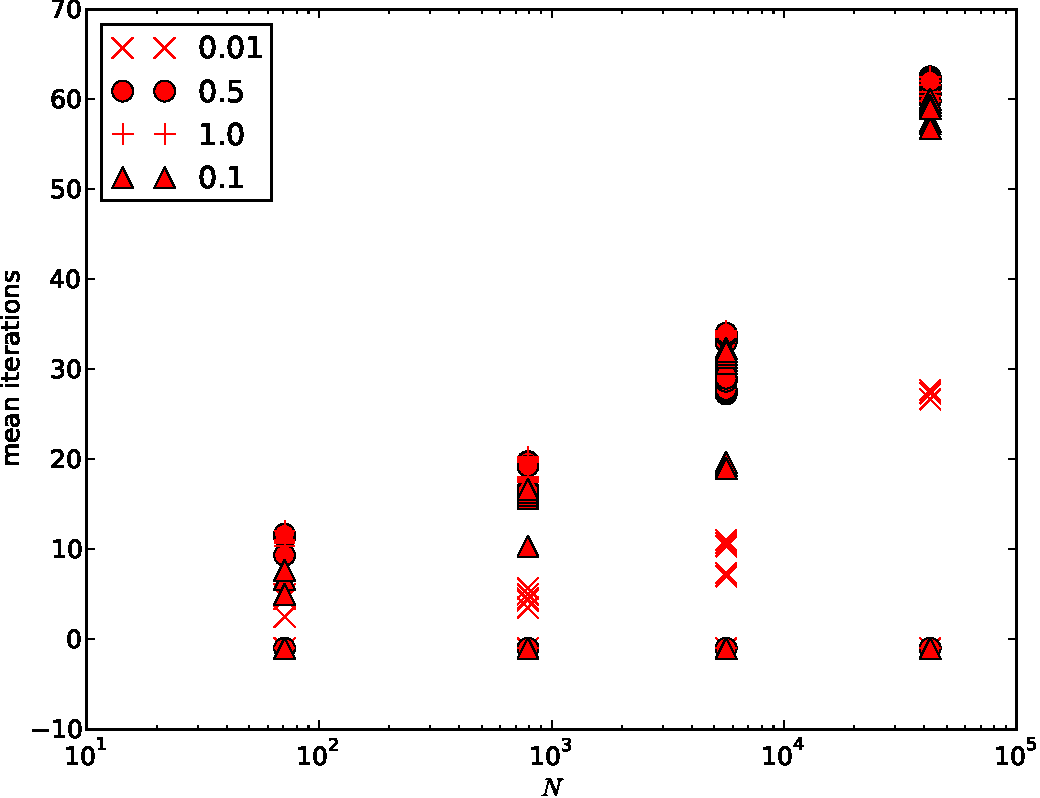
\includegraphics[width=0.8\textwidth]{plots/linear_solvers/ilu-1decoupleddummy-meanofnsolveritersvsinitialnnode.pdf}
  \caption{GMRES iterations to reach relerr $10^{-8}$ for the decoupled LLG preconditioned by ILU-1.}
  \label{fig:its-ilu-decoupled}
\end{figure}

\begin{figure}
  \centering
  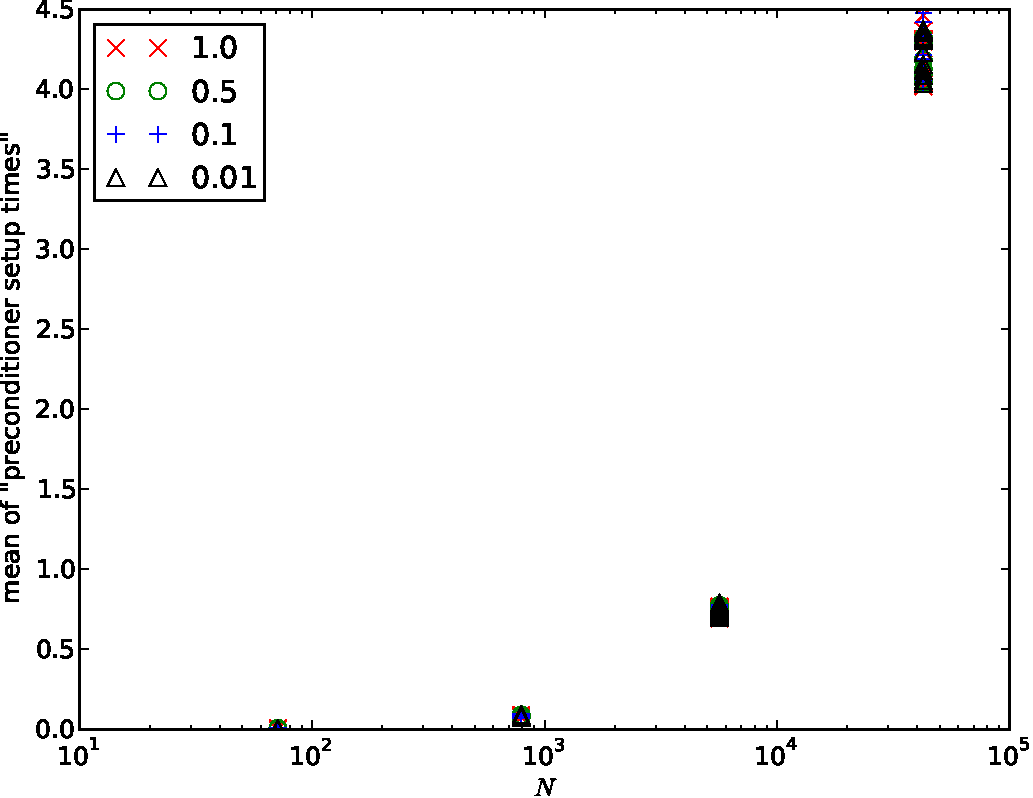
\includegraphics[width=0.8\textwidth]{plots/linear_solvers/ilu-1decoupleddummy-meanofpreconditionersetuptimesvsinitialnnode.pdf}
  \caption{Time to set up an ilu-1 preconditioner for the decoupled LLG block.}
  \label{fig:times-ilu-decoupled}
\end{figure}


Next we consider the preconditioner $\preca$, recall that this is essentially a direct solve without the dense block.
The iteration counts are shown in \cref{fig:its-p1-exact}, note that they are roughly independent of the number of nodes and vary only slightly with time step and the various other parameters.
However the preconditioner setup times, shown in \cref{fig:times-p1-exact} are not so good, as would be expected from a direct solve they grow rapidly for large systems.
Also, due to the direct solve, the memory usage of this preconditioner is large.
This is the reason for the missing data points for the largest $\Nn$: more than 16GB of memory was sometimes needed.

\begin{figure}
  \centering
  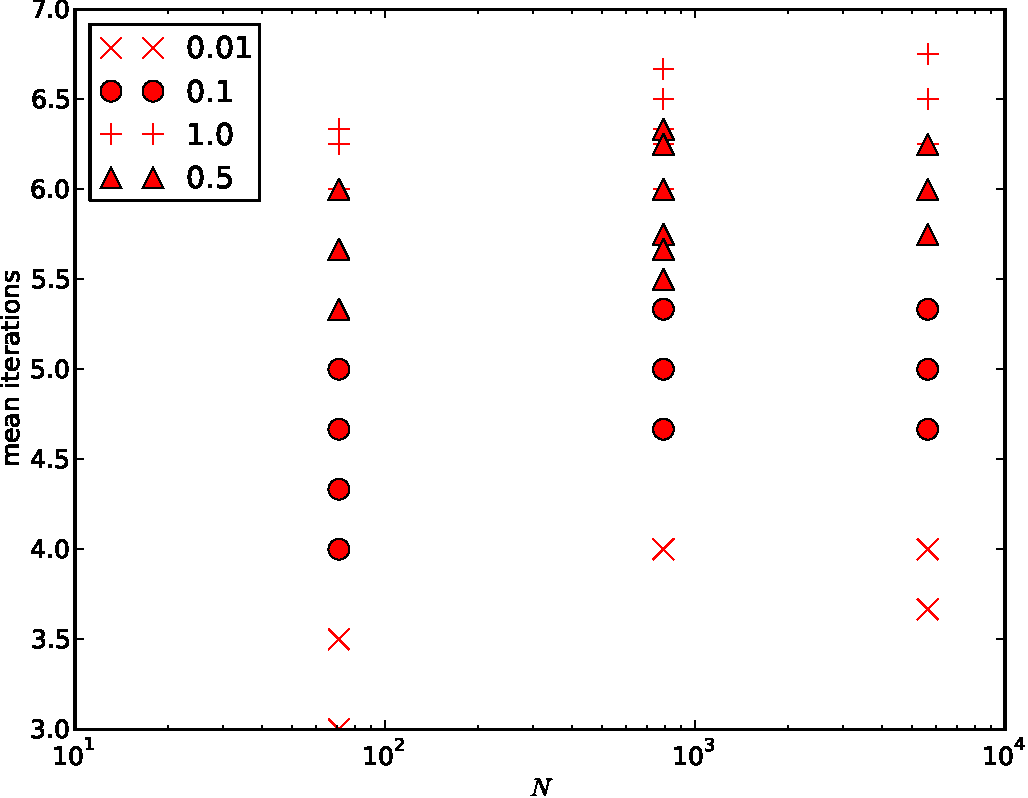
\includegraphics[width=0.8\textwidth]{plots/linear_solvers/som-main-exactimplicitdummy-meanofnsolveritersvsinitialnnode.pdf}
  \caption{Iterations for the monolithic system solved with $\preca$ inverted by LU decomposition, the legend indicates the time step size. Some data points for the largest $\Nn$ are missing due the LU factors requiring more than 16GB of memory.}
  \label{fig:its-p1-exact}
\end{figure}


\begin{figure}
  \centering
  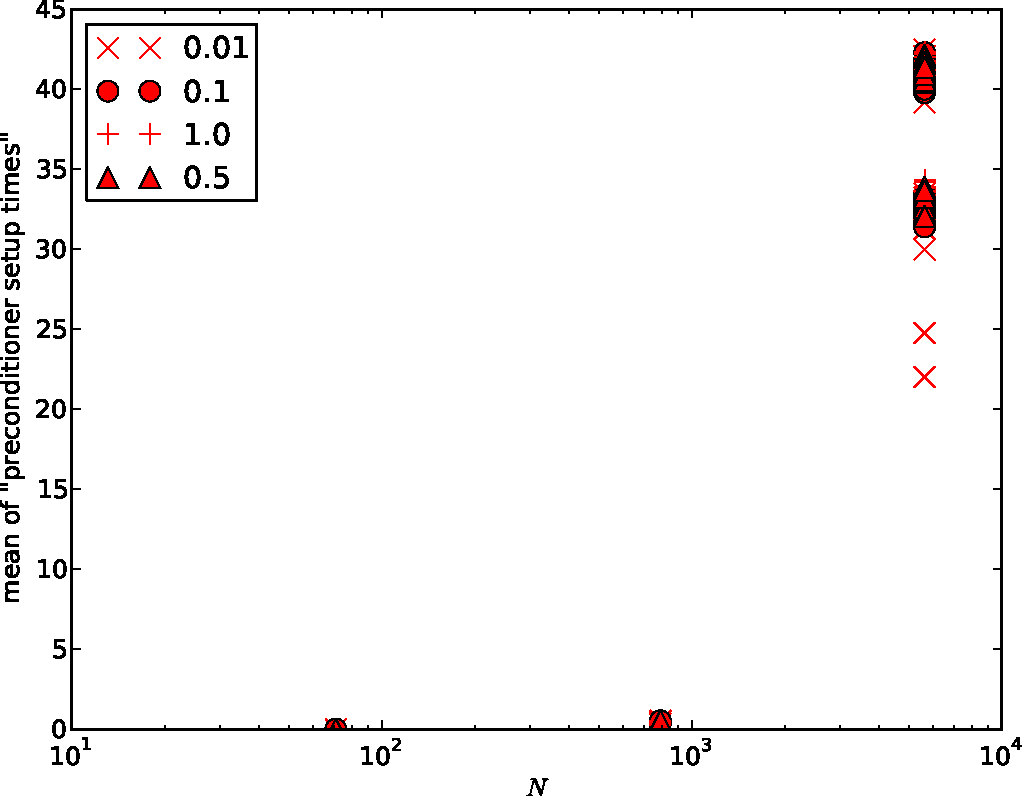
\includegraphics[width=0.8\textwidth]{plots/linear_solvers/som-main-exactimplicitdummy-meanofpreconditionersetuptimesvsinitialnnode.pdf}
  \caption{Preconditioner setup times for $\preca$ inverted by LU decomposition, the legend indicates the time step size. Some data points for the largest $\Nn$ are missing due the LU factors requiring more than 16GB of memory.}
  \label{fig:times-p1-exact}
\end{figure}

Now we consider the preconditioners $\parinexact{\precb}$ and $\parinexact{\precc}$, which were designed to reduce the setup time and memory issues of $\preca$ by greatly reducing the portion of the preconditioner which is solved directly.
The iteration counts are shown in \cref{fig:its-p23-exact}, we see that for both preconditioners the number of iterations increases only slightly as the number of nodes increases and that the various other parameters have little effect.
Also note that the iteration counts are not much larger than those of $\preca$.
The preconditioner setup times are shown in \cref{fig:times-p23-exact}, they are significantly smaller than those in \cref{fig:times-p1-exact} but still grow unacceptably large due to the direct solve of the $\Fm$ block.
Interestingly the use of nodal integration decreases the time required for the set of the preconditioner, this is likely due to the ``mass-lumping'' effect discussed in \cref{sec:local-nodal-integr}.
However it does not decrease the time sufficiently for the preconditioner to be viable for real-world usage on problems with number of nodes $\Nn \gtrsim 10^4$.
Also of note is that, unlike $preca$, the required LU decomposition fits within the 16GB of available memory for all parameters.

\begin{figure}
  \centering
  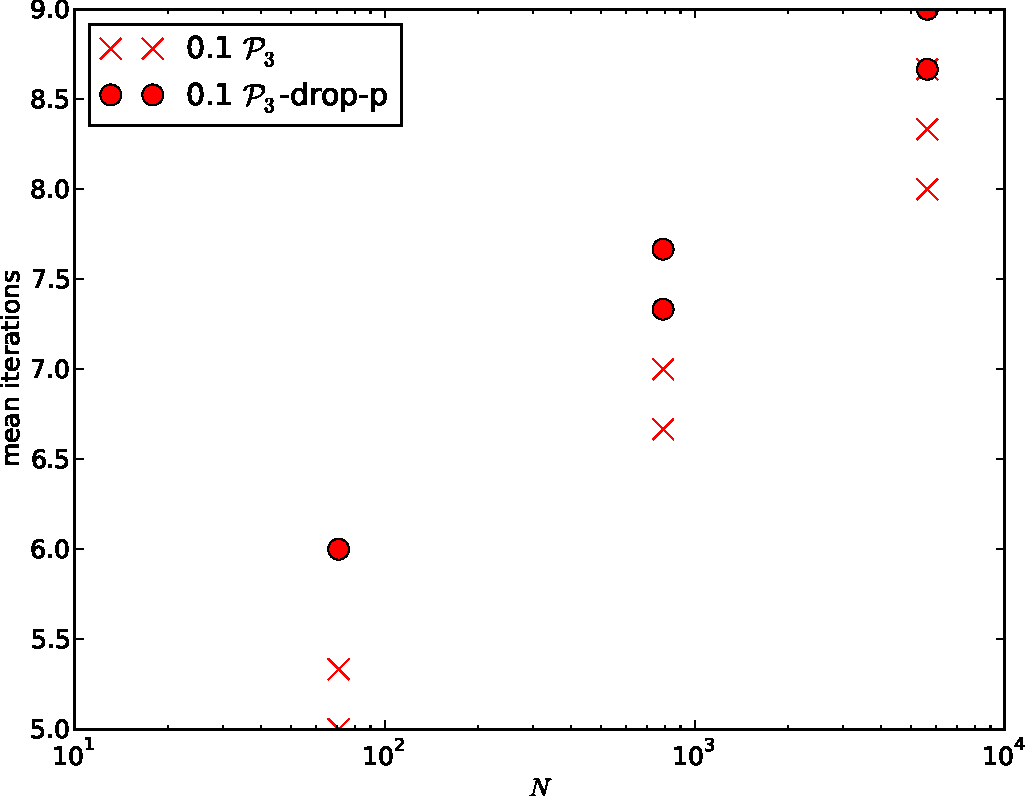
\includegraphics[width=0.8\textwidth]{plots/linear_solvers_p2p3/implicitexact-meanofnsolveritersvsinitialnnode.pdf}
  \caption{Iterations for the monolithic system with $\dtn=0.1$ preconditioned by $\parinexact{\precb}$ and $\parinexact{\precc}$.}
  \label{fig:its-p23-exact}
\end{figure}

\begin{figure}
  \centering
  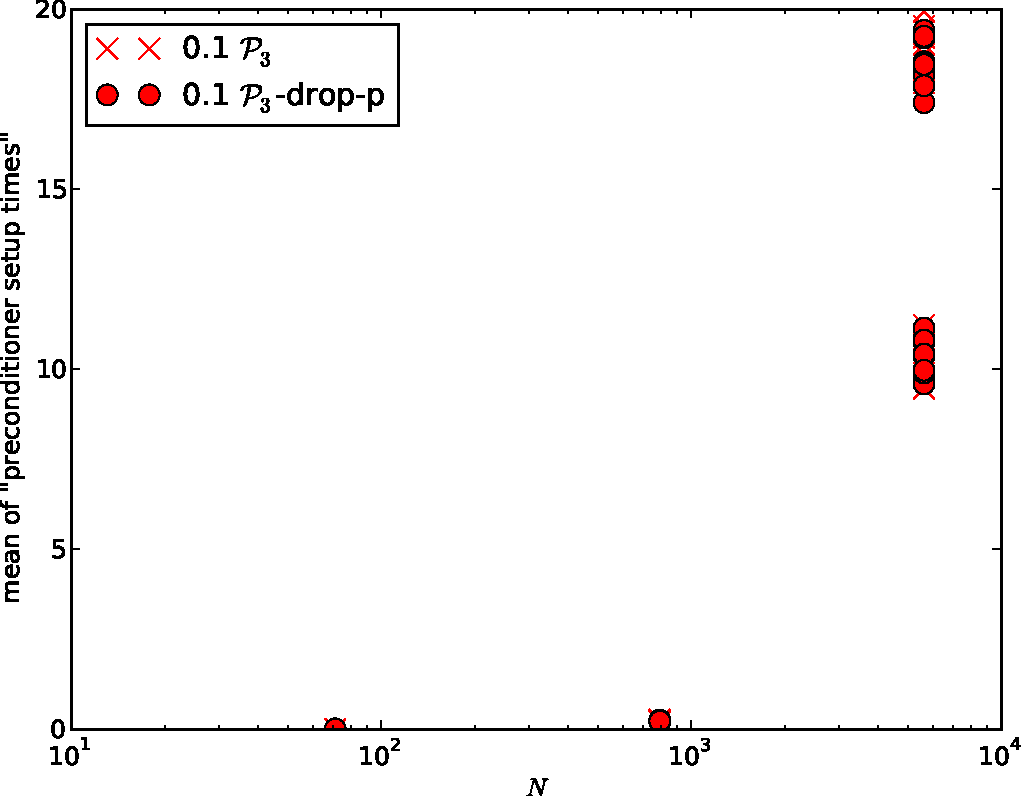
\includegraphics[width=0.8\textwidth]{plots/linear_solvers_p2p3/implicitexact-meanofpreconditionersetuptimesvsinitialnnode.pdf}
  \caption{Preconditioner setup times with $\dtn=0.1$ for $\parinexact{\precb}$ and $\parinexact{\precc}$ with $\Fm$ block inverted by LU decomposition and $\Am$ blocks approximated using AMG.}
  \label{fig:times-p23-exact}
\end{figure}


Finally we show iteration counts for the fully iterative preconditioners $\inexact{\precb}$ and $\inexact{\precc}$ where the $\Fm$ block is approximated using ILU-1.
We cannot expect $\Nn$-independent results here, since even the simpler case of the solution of the $\Fm$ block alone does not display such behaviour.
The iteration counts shown in \cref{fig:its-p23-ilu1}, are as expected: good at first but becoming ineffective for large number of nodes $\Nn$.
In particular, for the largest number of nodes GMRES did not converge within 400 iterations for any of the parameter sets.
Also of note is the much larger variation of the iteration counts with the problem parameters.
The preconditioner set up times, as shown in \cref{fig:times-p23-ilu1} are much better than when using the LU decomposition of the $\Fm$ block.

??ds try to find/show parameter dependency: some iteration counts are ok!

\begin{figure}
  \centering
  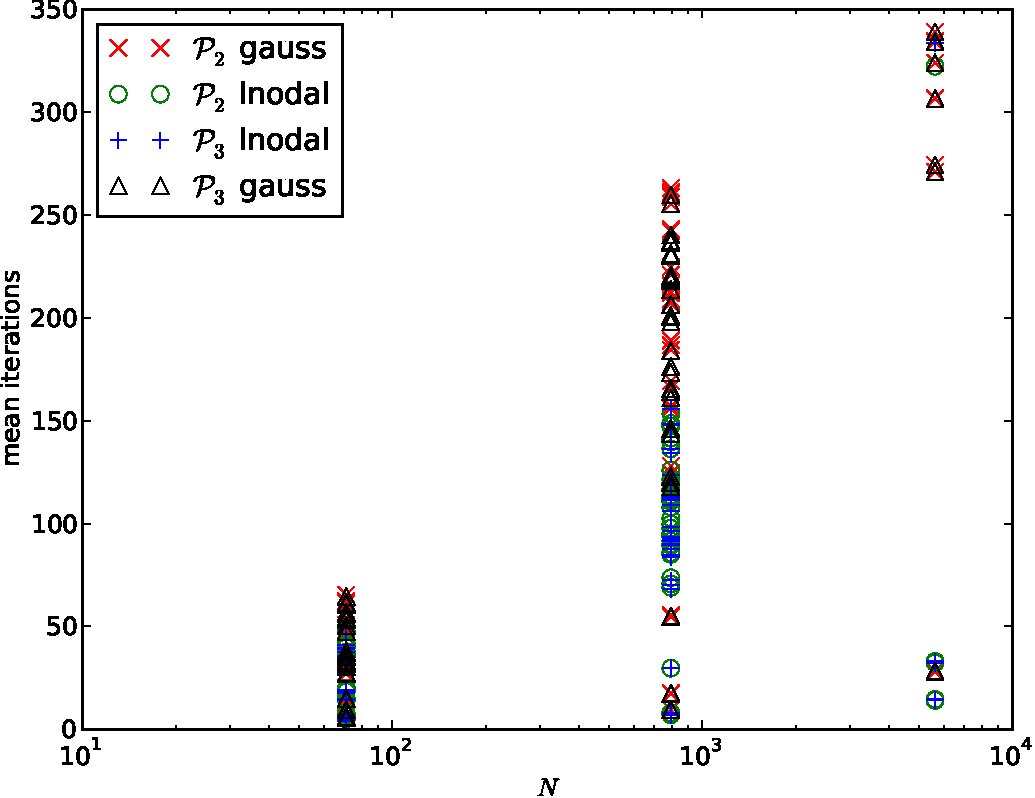
\includegraphics[width=0.8\textwidth]{plots/linear_solvers_p2p3/implicitilu-1-meanofnsolveritersvsinitialnnode.pdf}
  \caption{Iterations for the monolithic system with $\dtn=0.1$ solved with $\inexact{\precb}$ and $\inexact{\precc}$ with $\Fm$ block approximated by ilu-1 and $\Am$ blocks approximated using AMG. Some data points are missing for the largest $\Nn$ due to a lack of convergence.}
  \label{fig:its-p23-ilu1}
\end{figure}

\begin{figure}
  \centering
  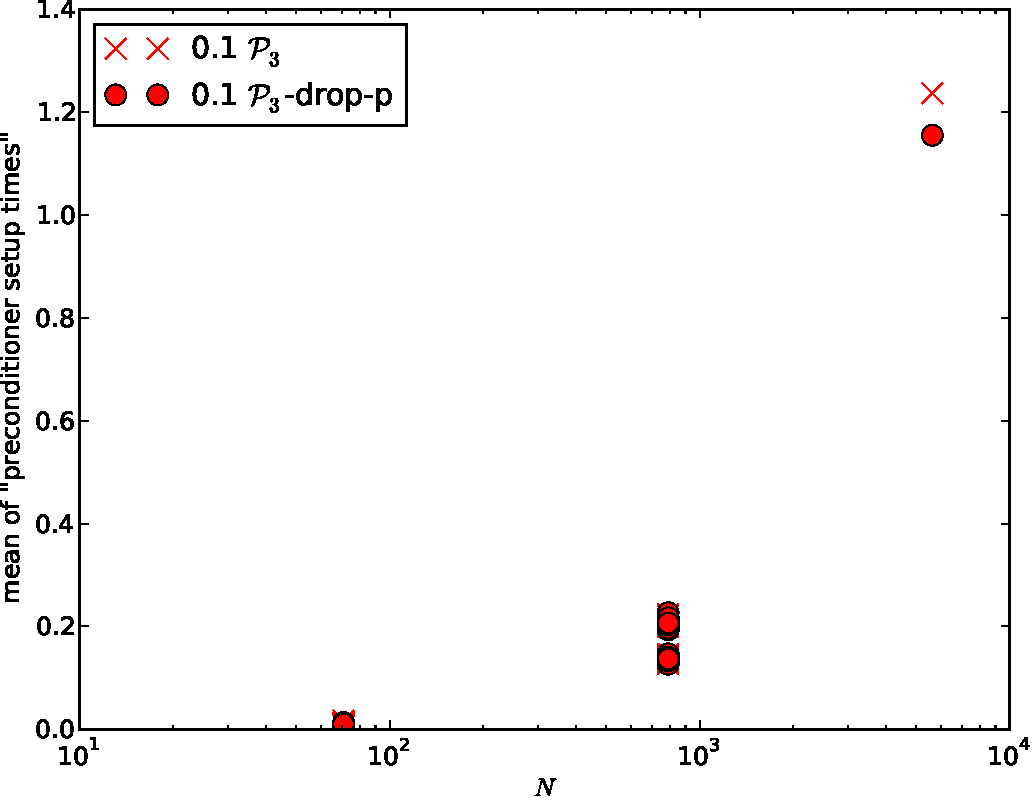
\includegraphics[width=0.8\textwidth]{plots/linear_solvers_p2p3/implicitilu-1-meanofpreconditionersetuptimesvsinitialnnode.pdf}
  \caption{Preconditioner setup times with $\dtn=0.1$ for the fully-iterative preconditioners $\inexact{\precb}$ and $\inexact{\precc}$. Some data points are missing for the largest $\Nn$ due to a lack of convergence.}
  \label{fig:times-p23-ilu1}
\end{figure}

??ds Effect of HLib? If time do this later


??ds if I get inner iteration preconditioner working then do this:
??ds maybe compare the total solve time for the semi-implicit method (with GMRES and ILU-1 preconditioning) and fully implicit method (with $\precb$, ILU-1 for the $\Fm$ block or maybe using BiCGstab for F?), both using HLib.
% Results are shown in \cref{fig:times-semi-vs-fully-implicit}, the fully implicit method is a little slower but not horrible..
% Note that in our current implementation the Jacobian assembly time for the fully implicit method is longer than that of the semi-implicit one, however this does not need to be the case with some simple optimisations discussed in \cref{sec:furth-optim-opport}.

% \begin{figure}
%   \centering
%   
\includegraphics[width=0.8\textwidth]{images/placeholder}
%   \caption{}
%   \label{fig:times-semi-vs-fully-implicit}
% \end{figure}


\section{Outlook}
\label{sec:furth-optim-opport}

We now compare the \emph{expected} performance of the fully implicit and decoupled approaches with the assumption that a ``sufficiently good'' preconditioner for the $\Fm$ block can be found and discuss further improvements that could be made.

In the fully implicit method timing results presented here the entire FEM Jacobian was recalculated at each Newton step (??ds timing results not in yet).
This is not actually necessary: the Poisson blocks, $\Am$, and LLG-Poisson coupling blocks, $\Qm$ and $\Pm$, (of \cref{eq:16}) are only dependent on the geometry (\ie the corresponding equations are linear), hence these blocks could be precomputed and stored.
This reduces the Jacobian assembly process for the fully implicit method to exactly that of the decoupled method.

As an aside: the mass matrix sub-blocks on the diagonal of the LLG-block ($\Mm$ of \cref{eq:llg-jacobian}) are similarly only dependent on the geometry.
Additionally the skew symmetric structure of \cref{eq:llg-jacobian} could be exploited so that the calculation of $\Km_x$ is reused for $-\Km_x$, and similarly for $\Km_y$ and $\Km_z$.
Applying these additional optimisations will reduce the Jacobian calculations to the assembly of three $\Nn \times \Nn$ Jacobian blocks and the magnetocrystalline anisotropy block (which will typically be either a single $\Nn \times \Nn$ block or empty, see \cref{sec:llg-jacobian}).


In practice the Newton residual assembly time is extremely small compared to the solve and Jacobian assembly times, so the difference due to assembling additional $\phim$ and $\phione$ residual components Newton steps after the first can be ignored.

We now examine the cost per Krylov iteration (or set of Krylov iterations for the decoupled case).
The monolithic approach has more non-zeros in the Jacobian (the P, Q, G blocks), giving approx $4 \Nn$ extra matrix elements, compared to a base of $11 \Nn$, hence approximately one third as much time again is taken for each Krylov step.
Also the fully coupled method must use GMRES for all blocks rather than only for $\Fm$ (with CG for the Poisson blocks), this requires a more computationally expensive orthogonalisation process.
This increase could possibly be removed by using BiCGstab rather than GMRES (see \cref{sec:krylov-solvers}).

Finally it is likely that the monolithic method will require more Krylov iterations to converge, but this depends on the preconditioner used for the $\Fm$ block.

??ds to combine all these need relative times for Jacobian assembly, krylov iters, gmres vs cg orthog, back subs...

Based on all these factors we can estimate that, with an effective preconditioner, the computational time for a monolithic time step should certainly be within a factor of 2 of the time for a decoupled step.


\section{Conclusions and future work}

We have demonstrated a fully implicit (monolithic) LLG-magnetostatics solver using preconditioned GMRES which is close in terms of cost per linear solve.
For medium numbers of nodes it appears that ILU-1 is a good preconditioner for the LLG block.
The partially-iterative preconditioners $\parinexact{\precb}$ and $\parinexact{\precc}$ are able to reduce the iteration count of GMRES extremely effectively and almost independently of the number of nodes.
However the fully-iterative equivalents, $\inexact{\precb}$ and  $\inexact{\preca}$, which use ILU-1 to approximate the LLG block are ineffective for more than a few thousand nodes (\ie matrices of size $\sim 10,000$).
As such cheap, effective and mesh independent approximations for the LLG block, $\Fm$, are still needed before the monolithic block-preconditioned method discussed here can be effective on large classes problems.

We have also demonstrated solvers for a decoupled LLG-magnetostatics solver, the time integration properties of this scheme have yet to be seen.


For granular or bit patterned media a domain-decomposition preconditioner exploiting the low/zero exchange coupling between grains/islands could make for a simple but effective domain decomposition preconditioner.
For example, such a preconditioner could be implemented by performing an independent direct solve on the matrix block associated with each grain/island and using this diagonal block solution as the preconditioner.
Since the number of nodes in a single grain/island is likely to be small this would remain effective even for very large numbers of grains/islands.

Reordering of the degrees of freedom, scaling, drop tolerance, fill-in level in the ILU preconditioner could be experimented with to allow the solution of larger systems or alternative parameters \cite[287]{Saad2000}.
However ILU is very unlikely to ever give $\Nn$-independent or parameter-independent results, so  it may not be worth experimenting extensively with such modifications.




%%% Local Variables:
%%% mode: latex
%%% TeX-master: "main"
%%% End:
